\PassOptionsToPackage{svgnames}{xcolor}
\documentclass[12pt]{article}



\usepackage[margin=1in]{geometry}  
\usepackage{graphicx}             
\usepackage{amsmath}              
\usepackage{amsfonts}              
\usepackage{framed}               
\usepackage{amssymb}
\usepackage{array}
\usepackage{amsthm}
\usepackage[nottoc]{tocbibind}
\usepackage{bm}
\usepackage{algorithm}
\usepackage[noend]{algpseudocode}
\usepackage{enumitem}
\usepackage{wrapfig}
\algdef{SE}[SUBALG]{Indent}{EndIndent}{}{\algorithmicend\ }%
\algtext*{Indent}
\algtext*{EndIndent}
  \newcommand\norm[1]{\left\lVert#1\right\rVert}
  \newcommand\TCP{\texttt{TCP} }
  \newcommand\UDP{\texttt{UDP} }
  \newcommand\IP{\texttt{IP} }
\setlength{\parindent}{0cm}
\setlength{\parskip}{0em}
\newcommand{\Lim}[1]{\raisebox{0.5ex}{\scalebox{0.8}{$\displaystyle \lim_{#1}\;$}}}
\newtheorem{definition}{Definition}[section]
\newtheorem{theorem}{Theorem}[section]
\newtheorem{notation}{Notation}[section]
\theoremstyle{definition}
\setcounter{tocdepth}{1}
\setcounter{section}{-1}
\begin{document}
\title{Revision notes - CS2107}
\author{Ma Hongqiang}
\maketitle
\tableofcontents

\clearpage
%\twocolumn
\section{Overview}
Security concerns with \textbf{deliberate} human actions that are designed to cause failure.
\begin{definition}[Security]
\hfill\\\normalfont Security is defined by the C-I-A triad.
\begin{itemize}
  \item Confidentiality: Prevention of unauthorised disclosure of information
  \item Integrity: Prevention of unauthorised modification of information or processes
  \item Availability: Prevention of unauthorised withholding of information or resources.
\end{itemize}
\end{definition}
It is difficult to achieve security due to
\begin{itemize}
  \item Security is not considered in design.
  \item Security requirements are difficult to be determined.
  \item There are many constraints in design the security features.
  \item There may exist implementation flaws.
\end{itemize}
Clearly, there is a trade-off between security and ease-of-use, performance and cost.
\clearpage
\section{Encryption}
\subsection{Definitions}
\begin{definition}[Encryption Scheme]
\hfill\\\normalfont An encryption scheme, or cipher, consists of two algorithms: \textbf{encryption} $E_k$ and \textbf{decryption} $D_k$, where $k$ is the key. \\
Suppose there is a plaintext $x$, $c:=E_k(x)$ is defined as ciphertext.
\end{definition}
\begin{theorem}[Properties of Encryption Scheme]
\hfill\\\normalfont An encryption scheme must meet the \textbf{correctness property}, that is
\[
\text{for any plaintext }x\text{ and key }k, D_k(E_k(x))=x
\]
Equivalently, $D_k\circ E_k=I$ the identity map.\\
It also needs to satisfy the security property, i.e., from the ciphertexts, it is difficult to derive useful information of the key $k$ and the plaintext $x$. Specifically, the ciphertexts should resemble sequences of random bytes.
\end{theorem}
Cryptography is the study of techniques in securin communication in the present of adversaries who have access to the communication. Some common placeholders used in cryptography are
\begin{itemize}
  \item Alice, usually the originator of message
  \item Bob, usually the recipient
  \item Eve, eavesdropper who can only listen
  \item Mallory, a malicious party who can modify messages
\end{itemize}
\subsection{Classical Ciphers}
\textbf{Remark}: Classical ciphers are not secure in the computer era.
\subsubsection{Substitution Ciphers}
\begin{definition}[Substitution Cipher]
\hfill\\\normalfont In substitution cipher, 
\begin{itemize}
  \item Plaintext: string over a set of symbols $U$.
  \item Ciphertext: string over a set of symbols $U$.
  \item Key: a substitution table $S$, which is an isomorphic function $S:U\to U$.\footnote{This guarantees the existence of the inverse function $S^{-1}$.}
\end{itemize}
\textbf{Encryption}: Given a plaintext string $X=x_1x_2\cdots x_n$ and key $S$, output the ciphertext
\[
E_S(X)=S(x_1)S(x_2)\cdots S(x_n)
\]
\textbf{Decryption}: Given a ciphertext string $C=c_1c_2\cdots c_n$ and key $S$, output the plaintext
\[
D_S(C)=S^{-1}(c_1)S^{-1}(c_2)\cdots S^{-1}(c_n)
\]
\end{definition}
The concept of key space is a general concept of encryption scheme.
\begin{definition}[Key space]
\hfill\\\normalfont \textbf{Key space} $\mathbb{S}$ is the set of all possible keys $k$. The \textbf{key space size} is the total number of possible keys $|S|$.\\
The \textbf{key size}(or \textbf{key length}) is the number of bits required to represent a key. It is given as $\lceil\log_2|S|\rceil$.
\end{definition}
For the substitution cipher from the set of alphabets and space character to itself, the key space size is $27!$ and key size is $94$.\\
In general, attacks have purpose to find the key or to obtain some information of the plaintext. Attacks requires access to some information beforehand. A simple and general attack method is \textbf{exhaustive search}.
\begin{definition}[Exhaustive Search]
\hfill\\\normalfont Exhasutive search examines all possible keys one by one. In the case of substitution cipher, given a ciphertext $C$ encrypted from a plaintext $X$,
\begin{algorithm}
\begin{algorithmic}
\For{each $S$ in key space $\mathbb{S}$}
  Compute $X'=D_S(C)$.
\If{$X'$==$X$} break; \EndIf
  \EndFor{Display $S$}
\end{algorithmic}
\end{algorithm}
\end{definition}
The running time of exhaustive search depends on teh size of key space $\mathbb{S}$. When key space size is large, exhaustive search becomes ineffective.\\
An efficient attack on substitution cipher is \textbf{known-plaintext-attack}.\\
\begin{definition}[Known-Plaintext-Attack]
\hfill\\\normalfont An attack is a known plaintext attack if adversary has access to pairs of ciphertext and their \textbf{corresponding} plaintexts, and tries to get the key.
\end{definition}
For substitution cipher, given a plaintext $X$ and ciphertext $C$, one can ontain directly entries in the table. Therefore, the key can be found given sufficiently long ciphertext, and substitution cipher is deemed not secure under known plaintext attack.\\
Even sometimes plaintexts are not readily available, they can be guessed.\\
Also, substitution cipher is vulnerable to \textbf{frequency analysis}, if the plaintexts is sentences of any language.
\subsubsection{Permutation Cipher}
\begin{definition}[Permutation Cipher]
\hfill\\\normalfont Permutation cipher is also known as transposition cipher.
\textbf{Encryption}: The plaintext is grouped into blocks of $t$ characters, and then applied a secret permutation to each block by shuffling the characters.
\textbf{Key}: the isomorphic function \begin{align*}
e:\{c_1,c_2,\ldots, c_t\}&\to\{c_1,c_2,\ldots, c_t\}\\
c_i&\mapsto p_i:=e(c_i)
\end{align*} 
We denote this permutation $p$ by
\[
p=(p_1,p_2,\ldots, p_t)
\]
The size $t$ is also part of the key and is kept secret. \\
\textbf{Decryption}: Apply $e^{-1}$ to $C$ to get $P$. 
\end{definition}
\textbf{Remark}: Permutation cipher also fails miserably under known-plaintext attack and is easily broken if plaintext is English text.
\subsubsection{One Time Pad}
\begin{definition}[One Time Pad]
\hfill\\\normalfont
\textbf{Key}: $n$-bit $k_1k_2\cdots k_n$.\\
\textbf{Encryption}: Given $n$ bit plaintext, apply key to get ciphertext
\[
C:=(x_1\oplus k_1)(x_2\oplus k_2)\cdots(x_n\oplus k_n)
\]
where $\oplus$ is the binary \texttt{XOR} operator.
\textbf{Decyption}: Given $n$ bit ciphertext, apply key to restore plaintext
\[
X=(c_1\oplus k_1)(c_2\oplus k_2)\cdots(c_n\oplus k_n)
\]
\end{definition}
This encryption scheme works because $\forall x, k, (x\oplus k)\oplus k = x$.
\textbf{Remark}: Although one-time-pad is unbreakable, the length of key is same as plaintext, which is useless in many applications.
\subsection{Modern Ciphers}
Modern ciphers generally refer to schemes that use computer to encrypt/decrypt, and their design take into considerations of plaintext attack and frequency analysis.\\
They are supposedly secure in a sense that any successful attack does not perform noticeably better than exhaustive search.\\
The security of an encryption scheme can be quantified by the \textbf{length of the key}, or more precisely $\lceil \log_2 N\rceil$ bits where $N$ is the number of searches required to break the cipher.
\subsubsection{Data Encryption Scheme}
Data Encryption Scheme has a key length of 56 bits. It can be broken using distributed computing or specialised chip.
\subsubsection{Stream Cipher and Initial Values}
\begin{definition}[Stream Cipher]
\hfill\\\normalfont Suppose plaintext has $M$ bits and secret key has $n$ bits. Stream cipher generates a $M$-bit sequence from the key, which is used as the secret key in the one-time-pad for encryption and decryption.
\end{definition}
\textbf{Remark}: Generator must be carefully designed so that it gives \textbf{cryptographically secure pseudorandom sequence}.
\begin{definition}[Stream Cipher with Initial Value]
\hfill\\\normalfont Most ciphers, like stream ciphers, have an initial value(IV). The initial value can either be randomly chosen or from a counter.\\
In stream cipher with IV, the $M$ bit pseudorandom sequence is generated from the secret key \textit{together} with IV. Final ciphertext contains the IV, \textit{followed by} output of the one-time-pad encryption.\\
For decryption, first extract IV. Generate pseudorandom sequence with key and extracted IV and decrypt the ciphertext.
\end{definition} 
\textbf{Remark}: In this case, initial value is known to everyone.\\
The purpose of IV here is to prevent leaking of \texttt{XOR}ed plaintexts, as without IVs, keys to encrypt the two plaintexts are the same, which causes \texttt{XOR}ed ciphertexts to be equal to \texttt{XOR}ed plaintext.
\subsubsection{Block cipher \& Mode-of-Operations}
Block ciphers are designed for some \textbf{fixed size} input/output. For example, AES is designed for 123 bits input/output.\\
For large plaintext, it is 
\begin{enumerate}
\item divided into blocks first, and
\item have block cipher applied
\end{enumerate}
The method of extension of encryption from a single block to multiple blocks is called \textbf{mode-of-operation}.
\begin{definition}[Electronic Code Block(ECB) Mode]
\hfill\\\normalfont Electronic Code Book is the most simple mode where it 
\begin{enumerate}
  \item Divide the plaintext into blocks, and
  \item applies block cipher to each block, \textbf{with the same key}.
\end{enumerate}
\end{definition}
\clearpage
\begin{figure}[h]
\centering
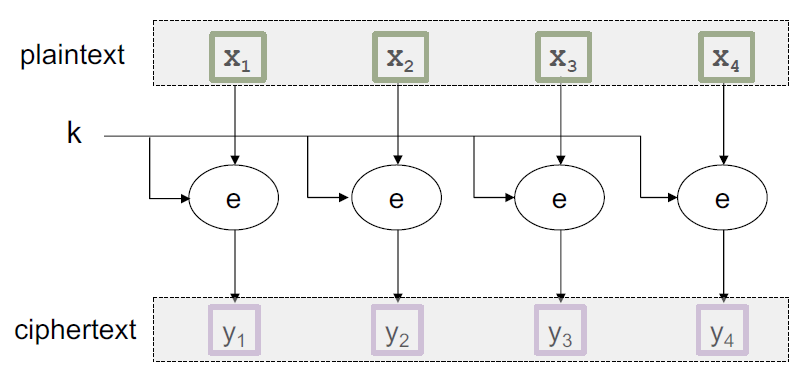
\includegraphics[width = 0.5\textwidth]{1_1.png}
\end{figure}
\textbf{Remark}: ECB might leak information on the plaintext, if a deterministic encryption scheme is used.\\
Cipher Block Chaining has additional mechanisms so that two blocks with the same content gives different ciphertext.
\begin{definition}[Cipher Block Chaining(CBC) mode]
\hfill\\\normalfont 
In cipher block chaining, the initial value will be used to generate first ciphertext block, which will be used as initial value of the next block.
\end{definition}
\begin{figure}[h]
\centering
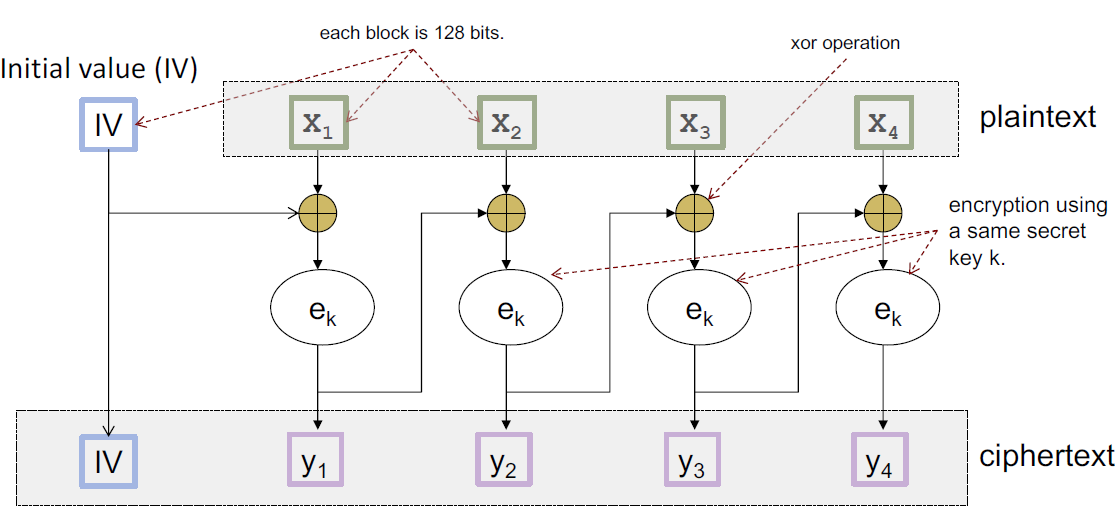
\includegraphics[width = 0.8\textwidth]{1_2.png}
\end{figure}
\subsection{Cryptography Pitfalls}
\subsubsection{Reusing IV/one-time-pad in Encryption}
Initial values is not secure if it is predictable.
\subsubsection{Keys Generation}
Numbers used to generate key must be pseudorandom for a computational perspective, like \texttt{java.security.SecureRandom}.
\subsubsection{Designing your own cipher}
The basic rule is to use existing scheme, and do not design own cipher.
\subsubsection{Reliance on Obscurity}
Generally, we need to adhere to \textbf{Kerckhnoffs' Principle}:
\begin{definition}[Kerckhoffs' Principle]
\hfill\\\normalfont A system should be secure even if everything about the system, except the secret key, is public knowledge.
\end{definition}
Security through obscurity, that is to hide the design of the system in order to achieve security, should be used to build a layered defense and should not be solely relied on.\\
In this module, we always assume that the attackers know the algorithms.
\clearpage
\section{Authentication}
\begin{definition}[Authentication]
\hfill\\\normalfont Authentication is the process of assuring that the communicating entity, or origin of a piece of information, is the one that it claims to be.
\end{definition}
For this course, authenticity implies integrity.\\
Authentication concerns communication channel, data, etc.
\subsection{Password}
In any password system, there are two stages.
\begin{enumerate}
  \item \textbf{Bootstrapping}: server and user establish a common password. Server keeps a file recording the \textit{identity} and \textit{password}.\\
  This is done by \begin{itemize}
  \item Server/user chooses a password and sends it to the user/server through another communication channel.
  \item Default password
\end{itemize}
  \item \textbf{Authentication}: server authenticates an entity. It the entity gives the correct password coressponding to the claimed identity, the entity will be deemed authentic.\\
  This can be done either with or without interactions. 
\end{enumerate}
\textbf{Remark}: Password is secret and only authentic user and server knows, whereas identity is not necessarily secret. In other words, the fact that an entity knows the password impliesthat the entity is either the server or the authentic user.
\begin{definition}[Weak Authentication]
\hfill\\\normalfont A weak authentication is one that subjected to the \textbf{replay attack}: information sniffed from the communicated channel can be used to impersonate the user.
\end{definition}
Password system is classified as a weak authentication.
\subsubsection{Attacks on Password System}
Password system may be compromised via
\begin{itemize}
  \item Attack on bootstrapping: Password can be intercepted during bootstrapping; attacker uses default password.
  \item Searching for password:
  \begin{itemize}
    \item Guessing password from social information
    \item Dictionary attacks
    \item Stealing password: shoulder surfing, sniffing, viruses, keylogger, login spoofing, phishing, spear phishing, etc.
  \end{itemize}
  \item Cache of shared workstation
  \item Insider attack
\end{itemize}
\subsubsection{Preventive measures}
Preventive measures to protect password include
\begin{itemize}
  \item Use strong password that is either \textbf{random}, \text{mix of special characters}.
  \item Password policies, which prevents weak passwords during bootstrapping and prevents dictionary attack/guessing by locking account after some failed attempts
  \item Layered protection on password files through \textbf{hashing}
\end{itemize}
\subsubsection{Security Questions}
Security question is viewed as a mechanism for \textbf{fallback authentication}, or a \textbf{self-services password reset}.\\
Choice of security questions need to be \textbf{memorable}, \textbf{consistent}, \textbf{nearly universal} and \textbf{safe}.\\
Scurity questions enhance ``usability'' at a cost of security.
\subsection{Biometric}
Biometric uses unique physical characteristics of a person for authentication. It consists of two stages:
\begin{enumerate}
  \item \textbf{Enrolment}: During enrolment, a template of an user's biometric data is captured and stored.
  \item \textbf{Verification}: During verification, biometric data of the person-in-question is captured and compared with the template using a \textit{matching algorithm}. The algorithm decides whether to accept or reject.
\end{enumerate}
Unlike password, there are possibilities of error, introducing the two rates below.
\[
\text{False Match Rate, FMR}=\frac{\text{number of successful false matches}}{\text{number of attempted false matches}}
\]
\[
\text{False Non Match Rate, FNMR}= \frac{\text{number of rejected genuine matches}}{\text{number of attempted genuine matches}}
\]
The \textit{matching algorithm} typically makes decision based on some adjustable threshold. Usually, there is a tradeoff between FMR and FNMR.\\
There are other types of errors:
\begin{itemize}
  \item Equal error rate: the threshold when FMR = FNMR.
  \item False-to-enroll rate: Some users' biometric data can't be captured during enrolment.
  \item Failure-to-capture rate: Biometric data may fail to be captured during authentication.
\end{itemize}
Biometric system is secure if the scanner and the communication channel to matching algorithm is secure. Additional protection may include liveness detection.\\
The following table contains some differences between biometrics and password.
\begin{table}[h]
\centering
\begin{tabular}{|c|c|}
\hline
Password&Biometric\\\hline
Can be changed&Cannot\\\hline
Need to remember&Don't have to\\\hline
Zero non-match rate&Probability of error\\\hline
Users can pass the password to others&Not possible\\\hline
\end{tabular}
\end{table}
\subsection{$n$-factor authentication}
$n$-factor authentication requires at least two different authentication factors, such as
\begin{itemize}
  \item Something you know, e.g., password
  \item Something you have, e.g., security token, mobile phone
  \item Who you are, e.g., Biometric
\end{itemize}
\subsubsection{One Time Password Token}
One Time Password Token is a hardware that generates one time password. Each token and the server share some secret keys used to generate the OTP by
\begin{enumerate}
  \item either \textbf{Time-based}: Based on the shared secret and current time interval, a password $K$ is generated which is known to both server and the user
  \item or \textbf{Sequence-based}: An event triggers the change of the password
\end{enumerate}
Examples of 2FA, like Password + OTP token, are given in the lecture notes and will be omitted here. \\
$n$-FA is secure if we assume that the reader, server and the channel of communication are all secure.
\clearpage
\section{Authenticity, MAC and Signature}
\subsection{Type of Cryptography}
\begin{definition}[Symmetric Key Cryptography]
\hfill\\\normalfont A symmetric key encryption scheme uses the same key for encryption and decryption, i.e.
\begin{align*}
c:&=E_k(m)\\
m=D_k(c)
\end{align*}
\end{definition}
A symmetric key cryptography is secure if it is difficult to get the plaintext from the ciphertext without the key.
\begin{definition}[Public Key Cryptography]
\hfill\\\normalfont A public key encryption scheme uses \textbf{public key} for encryption and \textbf{private key} for decryption, i.e.
\begin{align*}
c:&=E(k_\text{public}, m)\\
m&=D(k_\text{private}, c)
\end{align*}
\end{definition}
A public key cryptography(PKC) is secure if it is difficult to get either the plaintext or the private key from the ciphertext and public key.\\
One benefit of public key cryptography allows reduction of number of keys used. It also allows establishment of secure channel if one party publishes its public key.\\

Popular PKC schemes include RSA, which has a key size of 2048 bits, and ElGamal.\\
Detailed implementation of classroom RSA is covered in \texttt{GEH1036.pdf}.\\
Classroom RSA is \textit{not} secure; the standard for RSA is PKCS\#1.\\

Even for the standard RSA, it has the following problem:
\begin{itemize}
  \item RSA is much less time efficient compared to AES.
  \item RSA is not necessarily secure since
  \begin{enumerate}
    \item It is not known whether getting plaintext from ciphertext and public key is as difficult as getting the private key by prime factorisation.
    \item Homomorphic property of RSA can used to exploit RSA itself.
  \end{enumerate}
\end{itemize}
The performance issue can be resolved by
\begin{enumerate}
  \item Use PKC to establish a symmetric key cryptography key $k$.
  \item Use $k$ and Symmetric Key Cryptography to encrypt the file.
\end{enumerate}
\section{Hash}
\subsection{Hash with No Secret}
\begin{definition}[Hash]
\hfill\\\normalfont A cryptographic hash is a function that takes an arbitrarily large message as input and outputs a fixed size \textbf{digest}, and observe the following security properties:
\begin{itemize}
  \item Collision-resistant: It is difficult to find two different messages $m_1$ and $m_2$ that hash to the same digest, i.e. $h(m_1)= h(m_2)$.
  \item One-way: Given a digest $d$, it is difficult to find a message $m$, such that $h(m)=d$.
\end{itemize}
In fact, $(1)\Rightarrow (2)$.
\end{definition}
\begin{definition}[Keyed-Hash(aka MAC)]
\hfill\\\normalfont A keyed-hash is a function that takes an arbitrarily large message \textbf{and a secret key} as input, and outputs a fixed size \textbf{mac}(message authentication code), and observes the following security property:
\begin{itemize}
  \item Without knowing the key, it is difficult to forge the mac.
\end{itemize}
\end{definition}
General hashes may not work well for cryptographic purposes. One example is CRC checksum.\\
Popular and secure hashes include SHA-2, SHA-3.\\
Popular and secure keyed-hashes include CBC-MAC and HMAC.
\subsection{Data Integrity/Authenticity without secret keys}
With (unkeyed) hash, the integrity of the file can be checked by the algorithm in the diagram below.
\begin{figure}[h]
\centering
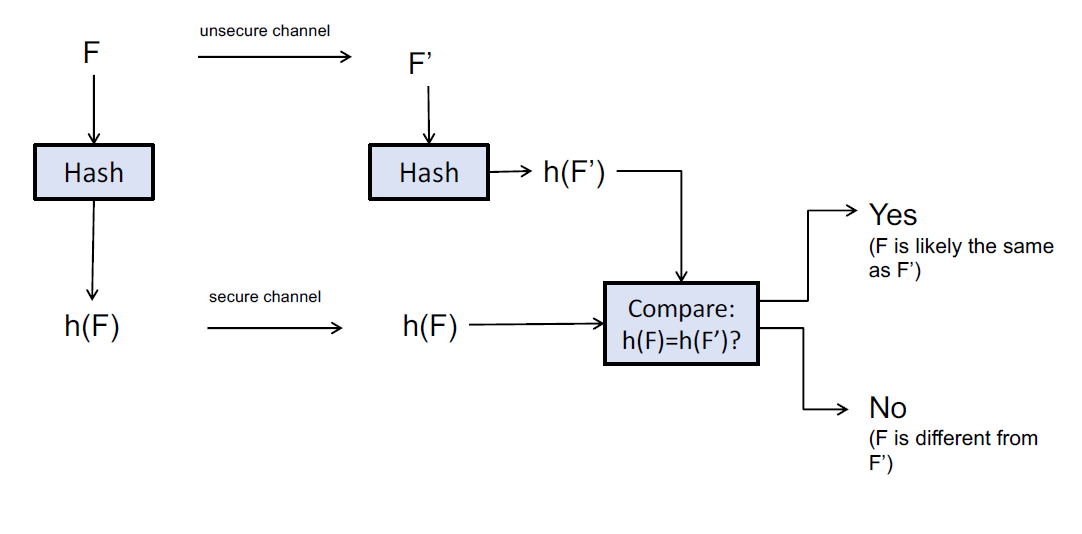
\includegraphics[width = 0.7\textwidth]{3_1.png}
\end{figure}
\textbf{Remark}: The assumption of secure channel for the \textbf{distribution of digest} is a must.
\subsection{Data Origin Authenticity with mac and Signature}
Data origin can be checked using mac following the algorithm in the next diagram.
\begin{figure}[h]
\centering
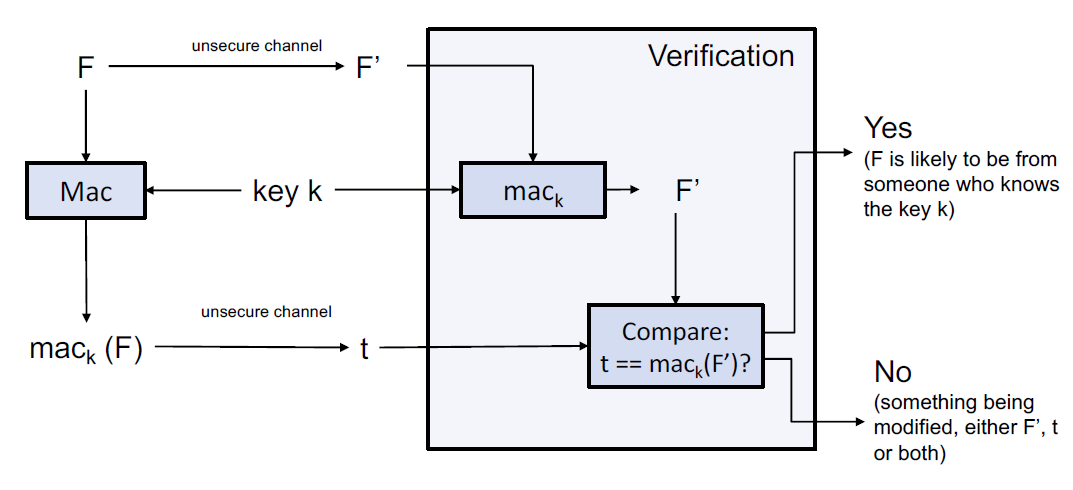
\includegraphics[width = 0.7\textwidth]{3_2.png}
\end{figure}
\textbf{Remark}: 
\begin{itemize}
\item We separate the concern of confidentiality from authenticity.
\item Usually mac is appended to $F$, and then transmitted. As such, mac is also called \textbf{authentication tag}.
\item The key must be sent to the verifier in a secure channel.
\end{itemize}
Data origin can alternatively be checked using digital signature, where symmetric key $k$ is replaced by a pair of public and private keys.
\begin{figure}[h]
\centering
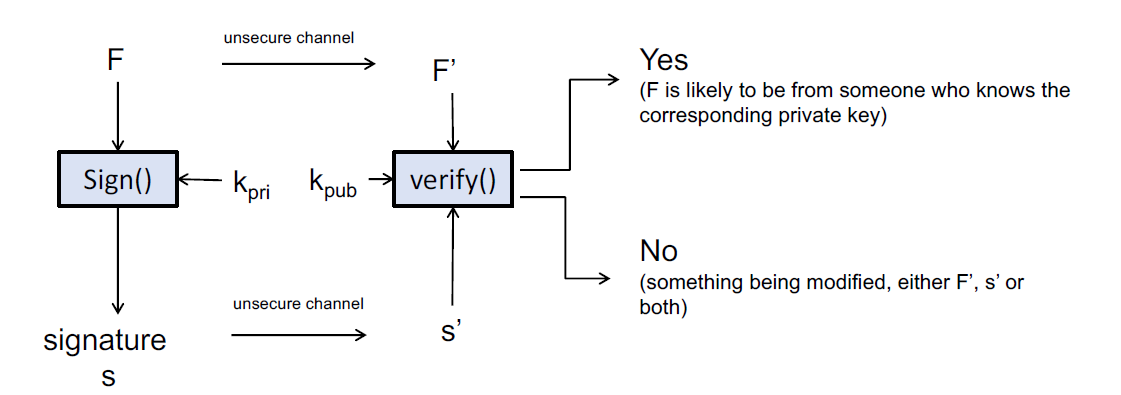
\includegraphics[width = 0.7\textwidth]{3_3.png}
\end{figure}
Signature is better in achieving authenticity compared to mac since it achieves \textbf{non-repudiation}, which means that, no one, except the authentic signer, can forge the signature.\\
Popular signature schemes include RSASSA-PSS and DSA(Data Signature Algorithm).
\subsection{Some Pitfalls}
Still, due to the reduced size of digest, it is subject to birthday attack, where it is quite likely to generate a collision from a pool of (file, hash) pairs. \\
Therefore, we require the length of the digest to be sufficiently large.\\
NIST reccomend key length for symmetric-key to be 112, and the recommended length of digest to be \textbf{at least} 224. 
\clearpage
\section{Public Key Distribution and Channel Security}
\subsection{Public Key Distribution}
For public key encryption scheme, we need a \textbf{secure channel} to distribute the secret key.\\
There are conventionally 3 ways to distribute these keys:
\begin{itemize}
  \item Public Announcement
  \item Publishing publicly available directory
  \item Publick Key Infrastructure
\end{itemize}
\subsubsection{Public Announcement}
The owner of publick key can broadcasts her public key via website, etc.\\
\textbf{Limitations}: not standardised and therefore there is not a systematic way to find/verify the public key when needed.
\subsubsection{Publicly Available Directory}
A server can be used to store and maintain the public keys of everyone.\\
\textbf{Limitations}: It is not easy to have a \textit{secure} public directory.
\subsubsection{Public Key Infrastructure and Certificate}
Public Key Infrastrcture(PKI) is a standardised system that distribute public keys. PKI is centered around two important components:
\begin{enumerate}
  \item Certificate Authority
  \item Certificate
\end{enumerate}
Public Key Infrastructure also provides a mechanism for ``trust'' to be extended, starting from the ``root''.
\subsection{Public Key Infrastructure}
Certificate Authority(CA) keeps a directory of public keys. CA also has its own public-private key pair. We assume that the CA's public key has been securely distributed to all entities involved.
\subsubsection{Certificate}
\begin{definition}[Certificate]
\hfill\\\normalfont A \textbf{certificate} is a digital document that contains at least the following 4 main itemz:
\begin{enumerate}
  \item The identity of an owner, for example, \texttt{alice@yahoo.com}
  \item The public key of the owner
  \item The time window that this certificate is valid
  \item The signature of the CA
\end{enumerate}
It also has additional information like the purpose of the public key.
\end{definition}
Certificate enables Bob to obtain Alice's public key and verifies its authenticity even without communicating with CA.
\subsubsection{Certificate Authority \& Trust Relationship}
Apart from \textbf{issuing certificate}, CA is also responsible to \textbf{verify that the information is correct}. This may involve manual checking.\\

CA also enstablishes a certificate chain:
\begin{itemize}
\item Most OS, browsers already have a few CA's public key pre-loaded. These are the ``root CA''.
\item Suppose Alice's certificate is issued by $CA1$, but Bob doesn't have public key of $CA1$.
\item In the first place, Alice who anticipates this, can send, along with her certificate, the $CA1$ certificate to Bob.
\item Bob then
\begin{enumerate}
\item verify $CA1$'s certificate using root CA's public key.
\item verify Alice's certificate using $CA1$'s public key.
\item verify Alice's email using Alice's public key.
\end{enumerate}
\item If Alice doesn’t attached $CA1$'s certificate, then Bob has to obtain it from other sources.
\end{itemize} 
Above working example illustrates the hierarchy of trust.
\subsection{Limitations and Attacks on PKI}
\subsubsection{Implementation Bugs}
One well-known implementation bugs is that some browsers ignore substrings in the name field after the null character when \textit{displaying} it but include them when \textit{verifying} the certificate.
\subsubsection{Abuse by CA}
A rogue CA can practically forge any certificate.
\subsubsection{Social Engineering}
Typo-squatting by changing some characters to some others which looks alike.
\subsection{Strong Authentication}
A weak authentication system, like \textit{password}, is subject to \textbf{replay attack}. Strong authentication can prevent replay attack by applying the \textbf{challenge-response} scheme.
\subsubsection{Strong Authentication under Symmetric Key Cryptography}
Suppose Alice and Bob have a shared key $k$, and have agreed on a message authentication code. The strong authentication can be carried out by
\begin{enumerate}
  \item Alice identifies herself by sending hello message to Bob
  \item Bob sends out \textbf{challenge}, which is a \textit{randomly} chosen plaintext $m$.
  \item Alice \textbf{responds} Bob with $t=\text{MAC}_k(m)$.
  \item Bob verifies $t$ is indeed the MAC of $m$.
\end{enumerate}
The secret key $k$ ensures the authenticity of Alice. The randomness of $m$ prevents the replay attack.\\
Such scheme where only Bob verifies Alice, but not vice versa is called \textbf{unilateral authentication}.
\subsubsection{Strong Authentication under Public Key Cryptography}
Suppose Alice wants to authenticate Bob,
\begin{enumerate}
  \item Alice \textbf{challenges} Bob with a random number $r$.
  \item Bob \textbf{responds} to the challenge by using his private key to sign $r$. Bob also attaches his certificate, in case Alice does not know his public key.
  \item Alice verifies Bob's certificate,  extracts Bob's public key from the certificate, and verifies that the signature is correct.
\end{enumerate}
Here, the value $r$ is also known as the \textbf{crypotgraphic nonce}.
\subsection{Key Exchange and Authenticated Key Exchange}
Strong authentication prevents the attack from eavesdropper, but does not prevent the malicious attacker. With authenticated key exchange, we can verify the authenticity as well as \textbf{establish a common key} between two parties.
\subsubsection{Key Exchange}
Under key exchange, we \textit{assume} authenticity and hope to achieve key establishment secure in the sense that eavesdropper fails. \\
One scheme is Diffie-Hellman key exchange, which achieve this purpose and \textit{forward secrecy}.\\
Following is a key exchange based on Public Key Cryptography.
\begin{enumerate}
  \item Alice generates a pair of private/public key.
  \item Alice sends the public key $k_e$ to Bob.
  \item Bob
  \begin{enumerate}
    \item Randomly chooses a secret $k$,
    \item Encrypts $k$ using $k_e$,
    \item Sends the ciphertext $c$ to Alice.
  \end{enumerate}
  \item Alice uses her private key $k_d$ to decrypt and obtain $k$.
\end{enumerate}
However, the above scheme fails when mallory presents, who can establishes 2 different key with Alice and Bob as the \textbf{man-in-the-middle}.\\

Therefore, to account for authenticity, we require \textbf{authenticated key exchange}. One such scheme is \textbf{station-to-station protocol}.
\subsection{Securing Communication Channel}  
Suppose a communication channel is subjected to sniffing and spoofing, the typical design in TLS to secure it is to 
\begin{itemize}
  \item Use \textbf{long-term keys} for handshake protocol, in order to establish \textbf{session keys}
  \item Subsequent communication is protected by session keys
\end{itemize}
Unilateral handshake is achieved in the following steps. Here, Alice wants to authenticate Bob.
\begin{enumerate}
  \item Alice obtains Bob's public key through PKI.
  \item Alice and Bob carry out \textbf{unilateral authenticated key exchange} protocol with Bob's public/private key.\\After authentication, Alice and Bob know \textbf{two} \textit{randomly} selected \textbf{session keys}: $t$ and $k$. $t$ is the secret key of a MAC, whereas $k$ is the secret key of a symmetric-key encryption like AES.
  \item Subsequent communication between Alice and Bob will be protected by $t$, $k$ and a \texttt{sequenceNumber}.\\ Suppose $m_1,\ldots, m_n$ are the sequence of messages exchanged, the actual data to be sent for $m_i$ will be
  \[
E_k(i\oplus m)\oplus \text{mac}_t(E_k(i\oplus m))
  \]
\end{enumerate}
Here, the session keys $t$ and $k$ ensures freshness to prevent replay attack. \texttt{SequenceNumber} ensures integrity, preventing reordering and dropping. $E_k$ ensures confidentiality and $text{mac}_t$ of the encrypted message ensures authenticity.












\clearpage
\section{Terminologies}
Tutorial 1:\\
\begin{itemize}
  \item Cryptology: the study of codes, or the art of writing and solving them.
  \item Cryptanalysis: the study of analyzing information systems in order to study the hidden aspects of the systems.
  \item Cryptography: the practice and study of techniques for secure communication in the presence of third parties called adversaries.
  \item NSA: National Security Agency
  \item NIST: National Institute of Standards and Technology
  \item cryptograrphy backdoor: a mechanism whereby one can alter a specific algorithm,  providing the perpetrator with a means to break the resulting cipher in significantly less time than would normally be required.
  \item Key Escrow: an arrangement in which the keys needed to decrypt encrypted data are held in escrow so that, under certain circumstances, an authorized third party may gain access to those keys. 
  \item Decryption order:  legislation that requires individuals to surrender cryptographic keys to law enforcement.
  \item Whitfield Diffie: an American cryptographer and one of the pioneers of public-key cryptography.
  \item Ron Rivest: a cryptographer and an Institute Professor at MIT.
  \item Alice, Bob, Eve, Mallory, Trent
  \begin{itemize}
    \item Alice and Bob: The original, generic characters. Generally, Alice and Bob want to exchange a message or cryptographic key.
    \item Eve: Evesdropper, who is usually a passive attacker. While she can listen in on messages between Alice and Bob, she cannot modify them. 
    \item Mallory: A malicious attacker who is active and who can modify messages, substitute messages, or replay old messages.
    \item Trent:  A trusted arbitrator, who acts as a neutral third party.
  \end{itemize}
\end{itemize}
Tutorial 2:\\
\begin{itemize}
  \item Graphical Passwords: an authentication system that works by having the user select from images, in a specific order, presented in a graphical user interface (GUI).
  \item Covert channel:  a type of computer security attack that creates a capability to transfer information objects between processes that are not supposed to be allowed to communicate by the computer security policy.
  \item Side channel attack: any attack based on information gained from the physical implementation of a computer system, rather than weaknesses in the implemented algorithm itself (e.g. cryptanalysis and software bugs)
  \item End-to-end encryption: a system of communication where only the communicating users can read the messages. The systems are designed to defeat any attempts at surveillance or tampering because no third parties can decipher the data being communicated or stored.
\end{itemize}
Tutorial 3:\\
\begin{itemize}
  \item Single Sign-On(SSO): A user logs in with a single ID and password to gain access to a connected system or systems without using different usernames or passwords, or in some configurations seamlessly sign on at each system.
  \item hardware random number generator: (true random number generator, TRNG) is a device that generates random numbers from a physical process, rather than a computer program. Such devices are often based on microscopic phenomena that generate low-level, statistically random "noise" signals, such as thermal noise, the photoelectric effect, involving a beam splitter, and other quantum phenomena.
  \item Quantum random Number Generator: a hardware random number generator that uses quantum phenomena.
  \item Authenticated encryption (AE) and authenticated encryption with associated data (AEAD, variant of AE) is a form of encryption which simultaneously provides confidentiality, integrity, and authenticity assurances on the data. 
  \item Retinal vs. Iris scan
\end{itemize}
\end{document}